\documentclass{beamer}
\usetheme{Berkeley}
\usecolortheme[RGB={132,184,24}]{structure} 
\usepackage[utf8x]{inputenc}
\usepackage{ucs}
\usepackage{amsmath}
\usepackage{amsfonts}
\usepackage{amssymb}
\usepackage{enumerate}
\usepackage{listings}
\logo{\pgfimage[width=15.7mm]{tudo127x97.jpg}}
\title{Einführung WS11/12}
\begin{document}

\section{Willkommen}
\begin{frame}{Willkommen}
\begin{center}
\huge
WebTech I - Blatt 2
\vspace{7mm}
\pgfimage[width=7cm]{ringe.jpg}

\end{center}
\end{frame}

\begin{frame}{Einführung}
\begin{center}Thema: JavaScript und DOM-Scripting\end{center}
\begin{itemize}
\item Aufgabe 2.1: Clientseitige Formularvalidierung
\item Aufgabe 2.2: Dynamisches Erweitern von HTML-Dokumenten
\item Aufgabe 2.3: Tooltip-Fenster
\item Aufgabe 2.4: Tabellenzeilen in JavaScript dynamisch hervorheben
\end{itemize}
\end{frame}

\begin{frame}{Aufgabe 2.1}
\begin{center}
Implementierung einer clientseitigen Formularvalidierung mithilfe von JavaScript (innerhalb der HTML-Datei):\\
~\\~\\
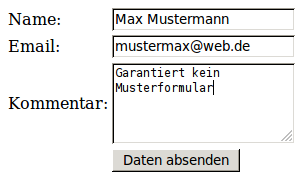
\includegraphics[width = 120px]{/home/maik/Desktop/formvali.png}
\end{center}
\end{frame}

\begin{frame}{Aufgabe 2.1 - Aufbau des HTML Fragments}
\begin{block}{HTML}
dsfsdf
\end{block}

\end{frame}


\end{document}
